\documentclass{article}
\usepackage{tikz}

\begin{document}
\section*{Probabilities}
\subsection*{Single events}
When we do an experiment, many different outcomes may happen. The \textit{likelyhood} of a certain
outcome is the probability of that outcome. It is measured from a scale of 0 to 1, where a 
probability of 0 means that that outcome is impossible, and a probability of 1 means that outcome
is the only one that is possible.

In short,
the probability of an event is written as $P(\textrm{event})$. Some examples follow:

$$ P(\textrm{the day after Friday will be Saturday}) = 1 $$
$$ P(\textrm{the Sun will rise in the west tomorrow}) = 0 $$
$$ P(\textrm{a pregnant mother will have a daughter}) = 0.5 = \frac{1}{2} $$

Let us consider the example of a coin toss. In a normal coin, there are two possible outcomes:
heads or tails. To \textit{experimentally} find the probability of either outcome, we will toss
the coin many times. We will record the outcomes in a table like below:

\begin{center}
	\begin{tabular}{ | c | c | }
		\hline
		Toss number & Outcome \\
		\hline
		1 & H \\
		2 & T \\
		... & ... \\
		\hline
	\end{tabular}
\end{center}

To find the probability of an outcome, the general formula for applying experimental results is:
$$ P(\textrm{outcome}) = \frac{\textrm{number of times outcome has occured}}
{\textrm{total attempts}} $$
So in our example, if we see that, out of 100 total attempts, there have been 50 heads and 50 
tails:

$$ P(\textrm{H}) = \frac{50}{100} = 0.5 $$
and,
$$ P(\textrm{T}) = \frac{50}{100} = 0.5 $$
Notice that, out of two probable outcomes, both have the same probability of ocurring. This means
the coin is random, i.e., if the coin is tossed there is an equal probability of either outcome.
Also notice that, the sum of all the outcomes equals 1: $0.5 + 0.5 = 1$. Furthermore, in such a
situation, where probabilities of all outcomes are equal, the outcomes are said to be perfectly
random.

However, if the result of our experiment yielded 75 heads and 25 tails, $P(\textrm{H}) = \frac{3}{4}
$ and $P(\textrm{T})=\frac{1}{4}$. The sum of all outcomes is still 1, yet the outcomes are not
all equal, meaning the coin is unfair and hence biased.

\newpage
\textbf{Problem.} In an experiment, a spinner of the following nature was used:

\begin{center}

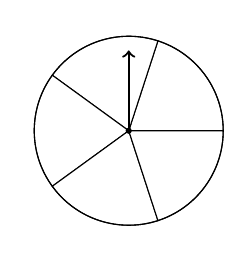
\begin{tikzpicture}[scale=0.6] % Adjusted scale for smaller size

% Define the number of slices
\def\numslices{5}

% Draw the spinner slices
\foreach \i in {1,...,\numslices} {
    \fill[fill=white,draw=black] (0,0) -- ({360/\numslices*(\i-1)}:2) arc[start angle={360/\numslices*(\i-1)}, end angle={360/\numslices*\i}, radius=2] -- cycle;
}

% Draw the circle for the spinner
\draw[] (0,0) circle(2);

% Draw the spinner arrow
\draw[->,black,thick] (0,0) -- (90:1.7);

% Draw the center dot
\filldraw (0,0) circle(1.5pt);

\end{tikzpicture}

\end{center}
Here, the arrow can be spun and it will land on one of the five segments. Each of the segments 
corresponds to a fruit: apple, banana, mango, jackfruit and lychee. The spinner was spun 50 times,
and it yielded the following results:

\begin{center}
	\begin{tabular}{ | c | c | }
		\hline
		outcome & number of times \\
		\hline\hline
		apple & 10 \\
		banana & 10 \\
		mango & 10 \\
		jackfruit & 10 \\
		lychee & 10 \\
		\hline
	\end{tabular}
\end{center}
Solve:
\begin{enumerate}
	\item Find the probability of the arrow landing on each of the fruits.
	\item Is the spinner fair or biased, explain.
\end{enumerate}

\subsection*{Multiple events}

Finding the probabilities of multiple events, happening one after another can involve two 
situations, where the events are dependent on each other and where the events are independent.

\subsubsection*{Independent events}

This involves events where no matter how many events occur, the probabilities of the individual
outcomes are unaffected. An example is multiple coin tosses. No matter how many times the coin is
tossed, the probability of the outcome being heads or tails is the same. 

To find the probabilities of multiple coin tosses, we may use tree diagrams.
\end{document}
